%!TEX root = bachelor.tex
\chapter{Theoretische Grundlagen}
\label{ch:theory}
In diesem Kapitel werden einige grundlegende Begriffe und Definitionen eingeführt, die in der folgenden Arbeit benötigt werden.
Zunächst wird auf die Definition eines Kegels, eines Kegelstumpfs und dessen Mantelfläche eingegangen.
%Anschließend wird eine Abbildung konstruiert, die die Oberfläche eines Kegels auf dessen Mantelfläche abbildet.
Anschließend wird kurz die Theorie linearer Ausgleichsprobleme erklärt, woraufhin der Prozess der Kamerakalibrierung
beschrieben wird.
Im Anschluss wird ein kurzer Überblick über Hough-Transformation zur Liniendetektion, sowie RANSAC zur Parameterschätzung gegeben.
Es werden Ellipsen definiert und beschrieben wie die kürzeste Distanz eines Punktes zu einer Ellipse approximiert werden kann.
Abschließend wird das Verfahren der Analytical Deformable Templates zur Detektion von parametrisierbaren Kurven erklärt.

\section{Kegel}
\label{s:cone}

\begin{definition}[Kegel]
	Ein Kegel ist ein geometrischer Körper, der durch eine beliebige Grundfläche, sowie einen Punkt (Spitze) definiert wird.
	Die Höhe $H$ eines Kegels ist definiert als die kürzeste Distanz der Spitze zur Grundfläche.
	Ein Kegel mit Kreis (auch Grundkreis genannt) als Grundfläche wird als Kreiskegel bezeichnet.
	Wenn die Grundfläche ein Zentrum besitzt, so wird die Verbindungslinie der Spitze mit diesem Zentrum als Achse des Kegels bezeichnet.
	Als gerade Kegel wird ein Kegel bezeichnet, dessen Grundfläche senkrecht zu seiner Achse steht \cite{James1992}.
\end{definition}

Im Folgenden werden nur gerade Kreiskegel betrachtet. Die Oberfläche eines Kegels mit Spitze $T(0,0,0)$, Radius $R$ und Höhe $H$, dessen Zentrum des Grundkreises in $(0,H,0)$ liegt, kann parametrisch beschrieben werden durch:
\begin{equation} \label{eq:paramCone}
\begin{aligned}
x &= \frac{u}{H} R~cos \theta \\
y &= u \\
z &= \frac{u}{H} R~sin \theta
\end{aligned}
\end{equation} %
mit $u\in [0, H]$ und $\theta \in [0, 2\pi)$. Hierbei steht $u$ für die aktuelle Höhe im Kegel. Um die vollständige Oberfläche zu beschreiben, muss $u$ das Intervall $[0, H]$ abdecken. Zu jedem $u$ ergibt sich ein Kreis mit Radius $\frac{u}{H} R$. Um einen vollständigen Kreis zu erhalten, muss $\theta$ demnach $[0, 2\pi)$ abdecken. Der Radius des Kreises nimmt zu bis er sein Maximum bei $u = H$ mit einem Wert von $R$ erreicht.

$S$ bezeichne die Seitenhöhe des Kegels und sei definiert durch das rechtwinklige Dreieck mit den Seitenlängen $H,R$ und $S$ (siehe Abbildung \ref{fig:cone}). Es gilt $S = \sqrt{H^2 + R^2}$.
\bigskip
\begin{definition}[Kegelstumpf und Ergänzungskegel]
	Ein Kegelstumpf entsteht aus einem Schnitt eines geraden Kreiskegels mit einer zur Grundfläche parallelen Ebene (siehe Abbildung \ref{fig:coneWithFrustum}) \cite{James1992}. 
	Der Kegel, der definiert ist durch die Schnittfläche und die Spitze des ursprünglichen Kegels, wird als Ergänzungskegel bezeichnet. 
	Der geometrische Körper zwischen Grundfläche und Schnittfläche wird als Kegelstumpf bezeichnet. 
	Die Grundfläche des Kegelstumpfs wird Grundkreis, die Schnittfläche Deckkreis genannt.

	$H, R, S$ sind dabei weiterhin die Höhe, Radius und Seitenhöhe des gesamten Kegels. Hinzu kommen $h,r,s$ als Höhe, Radius und Seitenhöhe des Ergänzungskegels. Die Höhe, sowie die Seitenhöhe des Kegelstumpfs werden durch die Differenzen $\Delta S = S - s,~ \Delta H = H-h$ charakterisiert (siehe Abbildung \ref{fig:coneFrustum}).
\end{definition}

\begin{figure}[!htb]
	\centering
	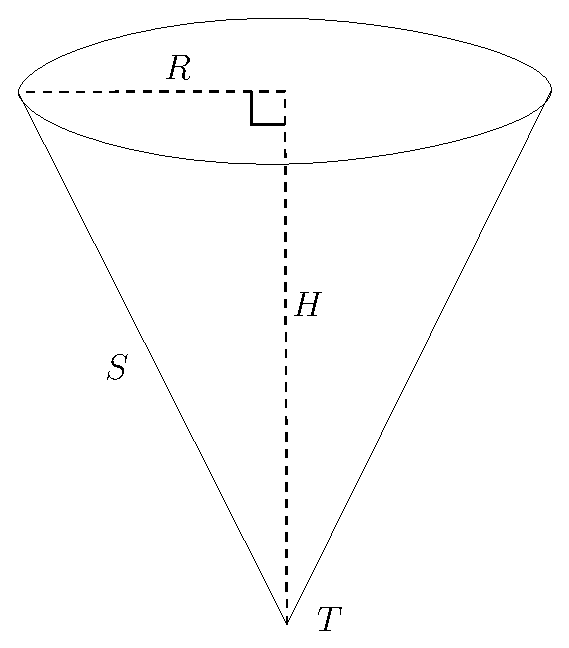
\includegraphics[scale=.5]{images/fullCone.eps}
	\caption{gerader Kreiskegel}
	\label{fig:cone}
\end{figure}

\begin{figure}[!htb]
	\centering
	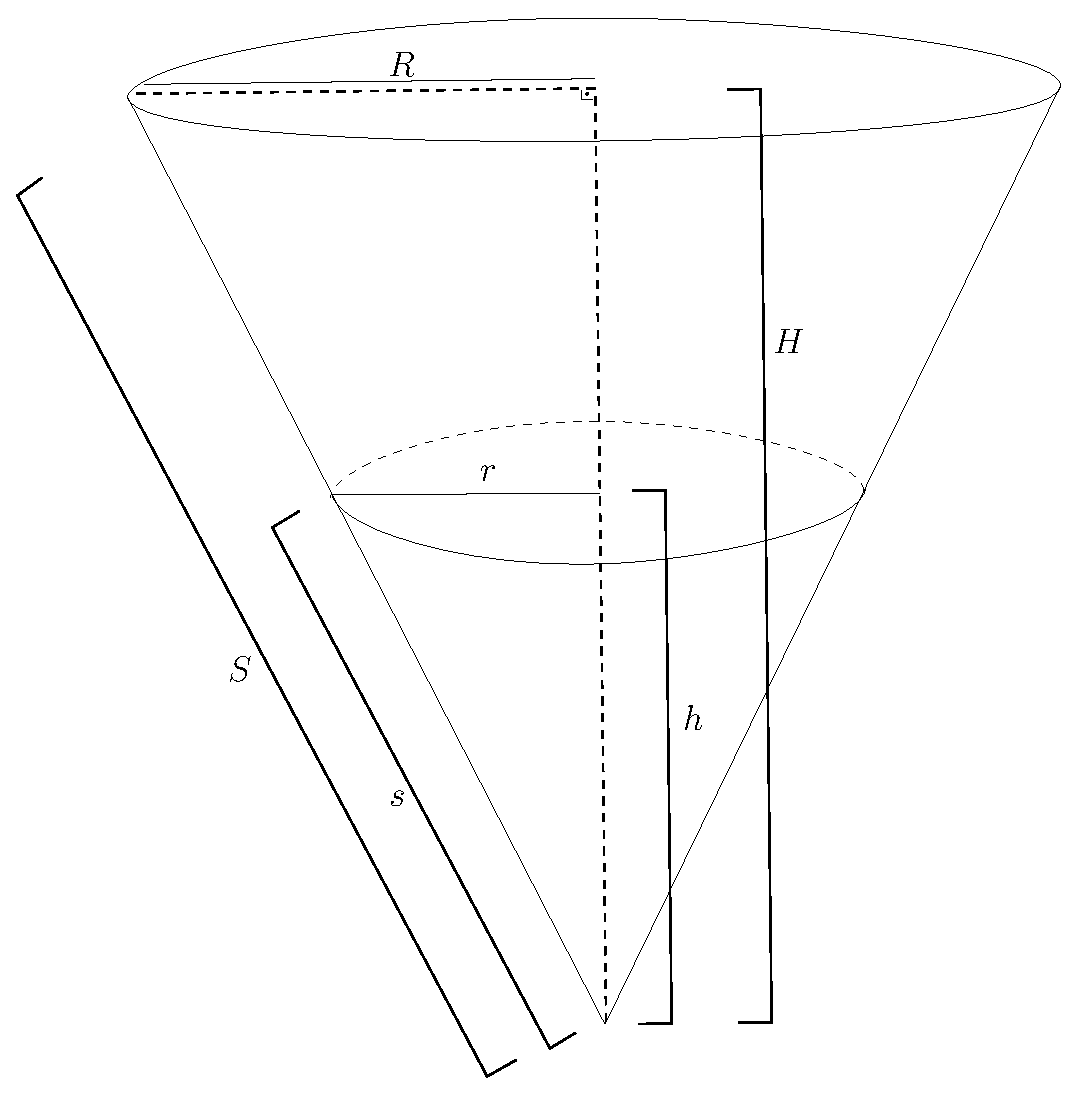
\includegraphics[scale=.4]{images/fullCone3.eps}
	\caption{Kegelstumpf und Ergänzungskegel}
	\label{fig:coneWithFrustum}
\end{figure}

\begin{figure}[!htb]
	\centering
	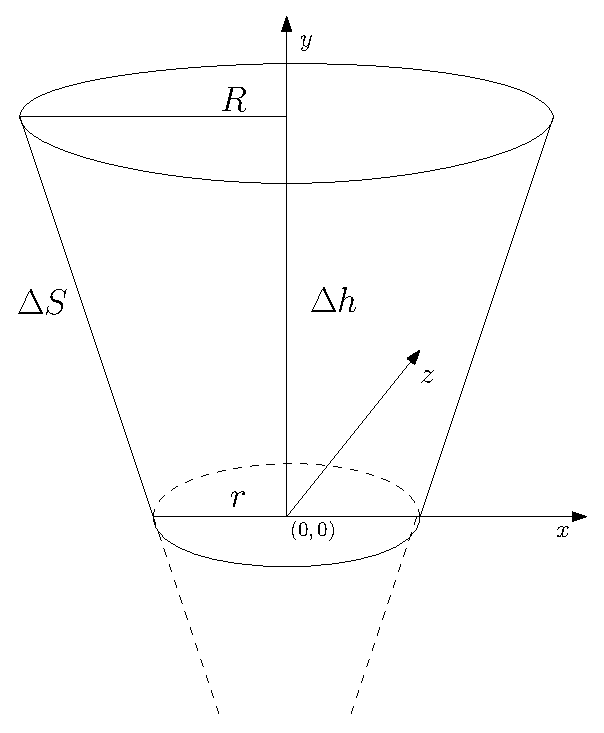
\includegraphics[scale=.7]{images/coneFrustum.eps}
	\caption{Kegelstumpf}
	\label{fig:coneFrustum}
\end{figure}

Die Oberfläche eines Kegelstumpfs mit Zentrum $(0,0,0)$ des Deckkreises und Zentrum $(0,\Delta H, 0)$ des Grundkreises wird analog zum klassischen Kegel durch folgende Parametrisierung definiert:
\begin{equation} \label{eq:paramFrustum}
\begin{aligned}
x &= (r + \frac{u}{\Delta H} (R - r))~cos \theta \\
y &= u \\
z &= (r + \frac{u}{\Delta H} (R - r))~sin \theta
\end{aligned}
\end{equation}
mit $u\in [0, \Delta H]$ und $\theta \in [0, 2\pi)$. Die parametrische Form eines Kegelstumpfs ist somit eine Verallgemeinerung der Parametrisierung von klassischen Kegeln (siehe Gleichung \ref{eq:paramCone}), wobei beim klassischen Kegel $r = 0$ gilt. Es wird eine Skalierung des Intervalls $[0, R]$ auf das Intervall $[r, R]$ durchgeführt, sodass ein Wert von $u = 0$ den Radius $r$ für den Deckkreis liefert.

Die Mantelfläche des Kegelstumpfs aus Abbildung \ref{fig:coneLateral} kann in Polarkoordinaten parametrisch beschrieben werden mit
\begin{equation} \label{eq:paramLateral}
\begin{aligned}
x &= -(s + \frac{u}{\Delta H}(S-s)) ~sin \phi \\
y &= ~~(s + \frac{u}{\Delta H} (S-s)) ~cos \phi,
\end{aligned}
\end{equation}
wobei  $u\in [0, \Delta H]$ und $\phi \in [0, \alpha) \subseteq [0, 2\pi)$. Die Seitenhöhen $s$ und $S$ gehören zum Ergänzungskegel, respektive zum ganzen Kegel.

\begin{figure}[!htb]
	\centering
	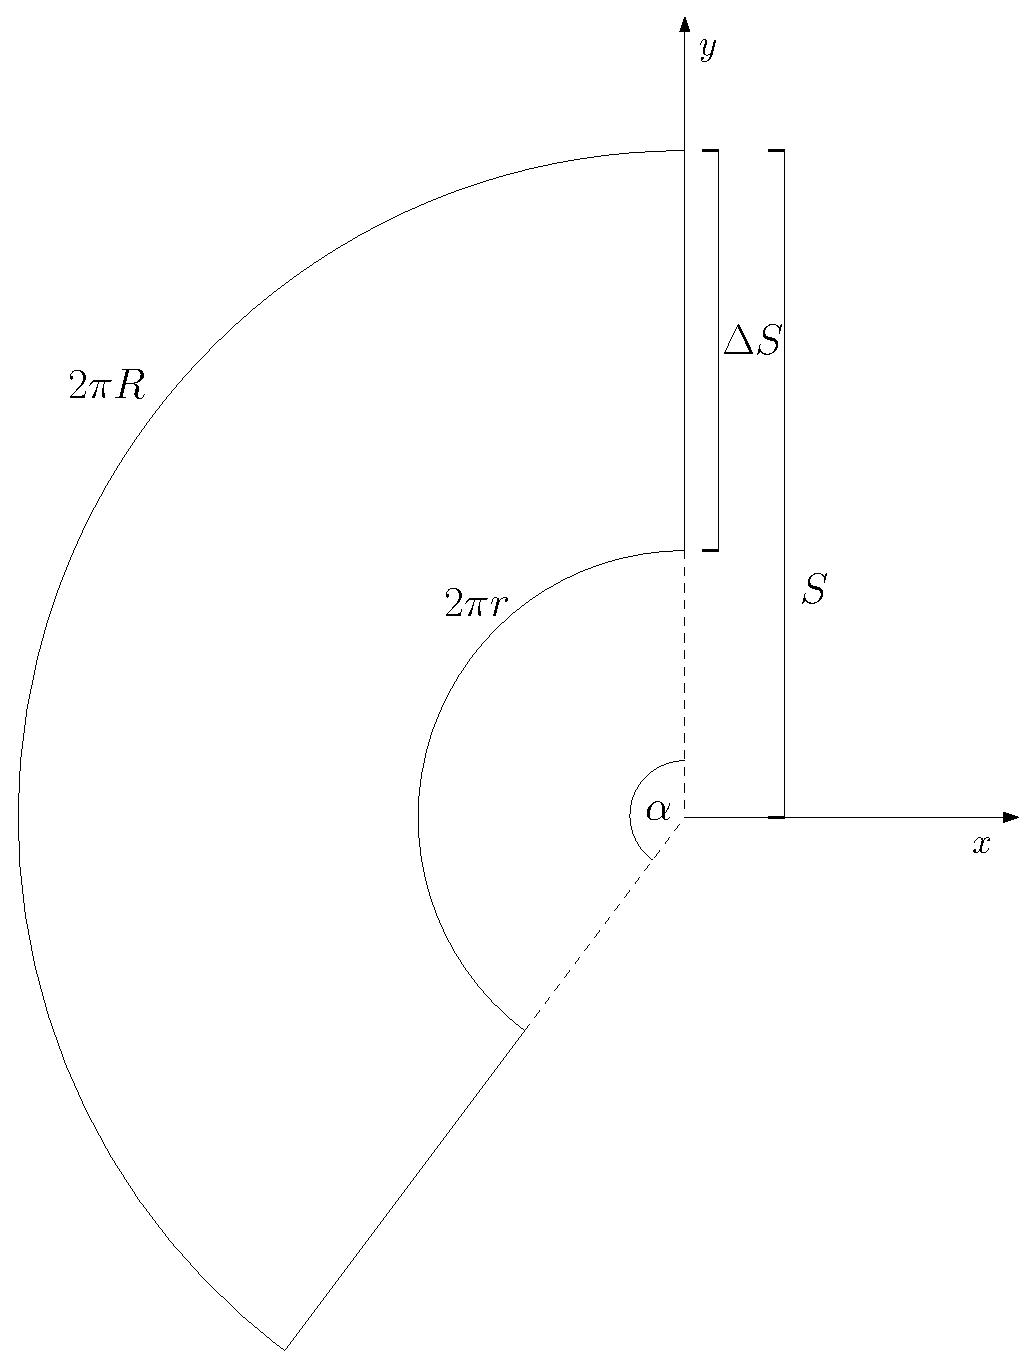
\includegraphics[scale=.4]{images/coneLateral.eps}
	\caption{Kegelmantelfläche}
	\label{fig:coneLateral}
\end{figure}

\FloatBarrier
Die Mantelfläche ergibt sich durch Entrollen des Kegelstumpfs. Da der Umfang des Kreises mit Radius $R$, $2\pi R$ beträgt, muss, wie in Abbildung \ref{fig:coneLateral} zu sehen, der äußere Kreisbogen die Bogenlänge $2\pi R$ haben. Analog beträgt die Bogenlänge des inneren Kreisbogens $2\pi r$. Für den Winkel $\alpha$ muss demnach gelten $\alpha S = 2\pi R$, also  $\alpha = 2\pi\frac{R}{S}$. Da sich die Seitenhöhe linear zur Höhe des Kegelstumpfs verhält, kann die Seitenhöhe durch die Höhe ausgedrückt werden. Hierbei gilt $(s + \frac{u}{\Delta H}(S-s))$. Bei Höhe $u = 0$ ergibt sich somit, wie erwartet, die Seitenhöhe $s$, bei Höhe $u = \Delta H$ die Seitenhöhe $S$.
%\begin{figure}[!htb]
%	\centering
%	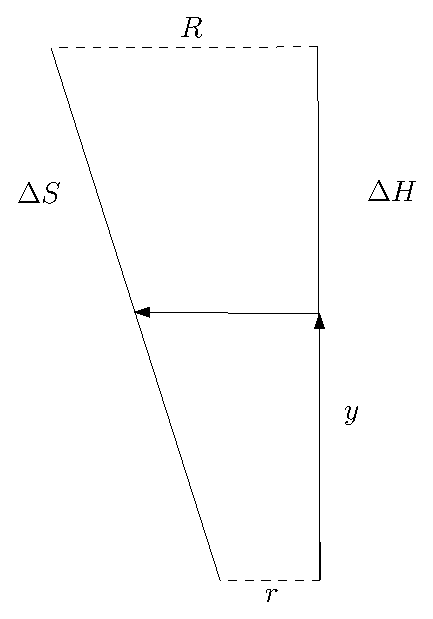
\includegraphics[scale=.7]{images/mapToLateralS.eps}
%	\caption{Abbildung der Kegelstumpfhöhe auf die Seitenhöhe.}
%	\label{fig:mapToLateralS}
%\end{figure}

Ein Punkt auf der Oberfläche des Kegelstumpfs kann eindeutig einem Punkt auf der Mantelfläche (und umgekehrt) zugeordnet werden. Dazu wird im Folgenden eine Abbildung und ihr Inverses konstruiert.

\subsection{Abbildung von Kegeloberfläche auf Mantelfläche}
Sei dazu ein Punkt $C(x,y,z)$ auf der Oberfläche des Kegelstumpfs gegeben. Gegeben durch die parametrischen Gleichung \ref{eq:paramFrustum}, hat $C$ die Form
\[
C(x,y,z) = \left(\left(r + \frac{u}{\Delta H} (R - r)\right)cos \theta, u, \left(r + \frac{u}{\Delta H} (R - r)\right)sin \theta\right)
\]  für ein $u\in [0, \Delta H]$ und $\theta \in [0, 2\pi)$.

Aus der $y$-Koordinate lässt sich direkt die Höhe $u$ ablesen und somit analog zur Gleichung \ref{eq:paramLateral} die zugehörige Seitenhöhe bestimmen. Diese entspricht dem Radius der Polarkoordinaten in der parametrischen Gleichung der Mantelfläche. Es wird hierfür eine Hilfsfunktion definiert:
\begin{equation} \label{eq:help1}
	T(y) := s + \frac{y}{\Delta H} (S-s).
\end{equation}


Da $R, r, \Delta H$  und nun auch die Höhe bekannt sind, kann der Winkel $\theta$ im Kegelstumpf ausgerechnet werden. Anschließend muss dieser noch mit  $\frac{R}{S}$ multipliziert werden, um ihn auf $[0, \alpha]$ zu skalieren (siehe Gleichung \ref{eq:paramLateral}).  In Gleichung \ref{eq:paramFrustum} wird nach $\cos\phi$, beziehungsweise nach $\sin\phi$ umgestellt und anschließend nach $\phi$ aufgelöst.
Zunächst werden beide Gleichungen durch $\left(r + \frac{y}{\Delta H} (R - r)\right)$ geteilt. Zu beachten ist nun, dass hier nicht die Umkehrfunktionen $\text{acos}$ oder $\text{asin}$ benutzt werden können, da $\sin$ und $\cos$ in einer Periode $[0, 2\pi)$ nicht injektiv sind. Die Wertebereiche der Umkehrfunktionen sind also eingeschränkt. Im Allgemeinen liefern sie nicht den erwünschten Winkel aus $[0, 2\pi)$.
Das gleiche Problem zeigt sich bei $\tan\phi = \frac{\sin\phi}{\cos\phi}$ und der Umkehrfunktion $\atano$. Um dieses Problem zu beheben, wird eine Fallunterscheidung gemacht und es ergibt sich wie folgt die sogenannte $\atant$-Funktion
\[
\atant(y,x) = 	\begin{cases}
					\atano \frac{y}{x} 					& \mbox{für } x > 0 \\
					\atano \frac{y}{x} + \frac{\pi}{2}	& \mbox{für } x < 0, y \geq 0 \\
					\atano \frac{y}{x} - \frac{\pi}{2}	& \mbox{für } x < 0, y < 0 \\
					\atano +\frac{\pi}{2}				& \mbox{für } x = 0, y > 0 \\
					\atano -\frac{\pi}{2}				& \mbox{für } x = 0, y < 0 \\
					0									& \mbox{für } x = 0, y = 0.
				\end{cases}
\]

Mit der Funktion wird untersucht in welchem Quadranten sich der Punkt $(x,y)$ befindet und entsprechend behandelt. Sie gibt den Winkel $\phi$ im Intervall $(-\pi, \pi]$ zurück.
Um den Winkel in $[0,2\pi)$ zu bestimmen, muss anschließend $\bmod~2\pi$ gerechnet werden.

Aus diesen Erkenntnissen wird wieder eine Hilfsfunktion definiert
\begin{equation} \label{eq:help2}
\Phi(x,y,z) := \frac{R}{S} \left[\left(\atant\left(\frac{z}{r + \frac{y}{\Delta H} (R - r)}, \frac{x}{r + \frac{y}{\Delta H} (R - r)}\right)\right) \bmod 2\pi \right],
\end{equation}
die den korrekten Winkel der Polarkoordinaten liefert und auf das Intervall $[0, \alpha)$ skaliert.

Mit den beiden Hilfsfunktionen \ref{eq:help1} und \ref{eq:help2}, sowie der Gleichung \ref{eq:paramLateral} ergibt sich insgesamt
\begin{equation}\label{eq:coneToLateral}
\begin{aligned}
\Psi \colon [r,R] \times [0, \Delta H] \times [r,R] &\to [s,S] \times [s,S]\\
\begin{pmatrix}
x \\ y \\ z
\end{pmatrix}  &\mapsto
\begin{pmatrix}
-T(y)\sin \Phi(x,y,z)\\
 ~~T(y)\cos\Phi(x,y,z)
\end{pmatrix}.
\end{aligned}
\end{equation}

\subsection{Abbildung von Mantelfläche auf Kegeloberfläche}

Analog lässt sich die Umkehrabbildung konstruieren.
Sei ein Punkt $L(x,y)$ auf der Mantelfläche des Kegelstumpfs gegeben. Aus der parametrischen Form der Mantelfläche (Gleichung \ref{eq:paramLateral}) ergibt sich

\[
L(x,y) = (-(s + \frac{u}{\Delta H}(S-s)) ~sin \phi, (s + \frac{u}{\Delta H} (S-s)) ~cos \phi)
\]

für ein passendes $u\in [0, \Delta H]$ und $\phi \in [0, \alpha) \subseteq  [0, 2\pi)$.

Da $L(x,y)$ in Polarkoordinaten gegeben ist, kann der Radius durch $\sqrt{x^2+y^2}$ bestimmt werden. Der Winkel $\phi$ mit inverser Skalierung $\frac{S}{R}$ kann analog zur Gleichung \ref{eq:help2} durch folgende Hilfsfunktion bestimmt werden:

\begin{equation}\label{eq:help3}
\Theta(x,y) := \frac{S}{R} \left[\left(\atant\left(-\frac{x}{\sqrt{x^2+y^2}}, \frac{y}{\sqrt{x^2+y^2}}\right)\right) \bmod 2\pi \right].
\end{equation}

Die Höhe des Kegels und somit auch der Radius lassen sich nun als Umkehrabbildung zur Hilfsfunktion \ref{eq:help1} bestimmen:
\begin{equation}\label{eq:help4}
\mathrm{H}(x,y) := \frac{\left(\sqrt{x^2+y^2}\right) - s}{S - s}\Delta H
\end{equation}

Insgesamt ergibt sich:
\begin{equation}\label{eq:LateralToCone}
\begin{aligned}
\Psi^{-1} \colon  [s,S]\times[s,S] &\to [r,R] \times [0, \Delta H] \times [r,R]\\
\begin{pmatrix}
x \\ y
\end{pmatrix} &\mapsto
\begin{pmatrix}
\left( r + \frac{\mathrm{H}(x,y)}{\Delta H} (R - r)\right)\cos\left(\Theta(x,y) \right) \\
\mathrm{H}(x,y)\\
\left( r + \frac{\mathrm{H}(x,y)}{\Delta H} (R - r)\right)\sin\left(\Theta(x,y) \right)
\end{pmatrix}
\end{aligned}
\end{equation}


\section{Lineares Ausgleichsproblem}
\label{s:LSQ}
Gegeben seien $m$ Messdaten $(x_1,y_1),\dotsc,(x_m,y_m)$, sowie eine lineare Funktion
\[
\varphi(x) = \sum_{i = 1}^{n}c_i\varphi_i(x)
\] %%
in $x$ mit Skalaren $c_1,\dotsc,c_n\in\mathbb{R}$, Funktionen $\varphi_1,\dotsc,\varphi_n$, $n\leq m$ und $n,m\in\mathbb{N}$.

Gesucht ist eine Lösung, welche die mittlere Abweichung

\[
\Delta_2 = \min_{c_1,\dotsc,c_n\in\mathbb{R}} \left(\sum_{j=1}^{m}\left(y_j - \varphi(x_j)\right)^2\right) = \min_{c_1,\dotsc,c_n\in\mathbb{R}} \left(\sum_{j=1}^{m}\left(\sum_{i=1}^{n}y_j-\left(c_i\varphi_i(x_j)\right)\right)^2\right)
\]

minimiert \cite{Stoer2007}.

Dieses Problem wird als lineares Ausgleichsproblem oder als Methode der kleinsten Quadrate bezeichnet und lässt sich wie folgt formulieren:

\[
\min_{c\in\mathbb{R}^n} ||y - Ac||_2
\]

mit
\[
\begin{aligned}
c &= (c_1,\dotsc,c_n)^T\in\mathbb{R}^n \\
x &= (x_1,\dotsc,x_m)^T\in\mathbb{R}^m \\
y &= (y_1,\dotsc,y_m)^T\in\mathbb{R}^m \\
A &= (a_{ij})\in\mathbb{R}^{m\times n} \rlap{\quad\text{mit}\quad $a_{ij} = \varphi_i(x_j)$}
\end{aligned}
\]

Das Problem lässt sich auch mit Hilfe der äquivalenten Normalengleichung
\[
	(A^TA)c = A^Ty
\]

lösen, wobei mindestens eine Lösung existiert und bei mehreren Lösungen, die Lösung mit kleinster 2-Norm ausgewählt wird.

Gilt darüber hinaus $\text{rang}\left(A\right) = n$ so ist $A^TA$ invertierbar und es gilt:

\begin{equation}\label{eq:normaleq}
c = \underbrace{(A^TA)^{-1}A^T}_{A^+}y.
\end{equation}

Dabei ist c die eindeutige Lösung mit kleinster 2-Norm. $A^+$ bezeichnet man auch als Moore-Penrose Inverse oder einfach als Pseudoinverse von $A$. Im Allgemeinen ist die Matrix $A^TA$ nicht invertierbar. Die Pseudoinverse kann somit nicht einfach mit $(A^TA)^{-1}A^T$ berechnet werden. Stattdessen lässt sie sich durch eine Singulärwertzerlegung (SVD) bestimmen \cite{Stoer2011}. Die Matrizen $A\in\mathbb{R}^{m\times n}$ und $A^+\in\mathbb{R}^{n\times m}$ können geschrieben werden als:

\[
\begin{aligned}
A &= U\Sigma V^T \\
A^+ &= V\Sigma^+U^T
\end{aligned}
\]

mit orthogonalen Matrizen $U\in\mathbb{R}^{m\times m}$ und $V\in\mathbb{R}^{n\times n}$ und einer Diagonalmatrix $\Sigma\in\mathbb{R}^{m\times n}$.
Die Diagonale der Matrix $\Sigma$ besteht aus den absteigend sortierten Singulärwerten von $A$, die Matrix $\Sigma^+\in\mathbb{R}^{n\times m}$ aus den jeweiligen reziproken Singulärwerten. Bei beiden Matrizen wird die Diagonale mit Nullen aufgefüllt.


Die Lösung des Ausgleichsproblems kann dann mittels SVD angeben werden als:
\[
c = \left(V\Sigma^+U^T\right)y
\]
Zu beachten ist, dass dieses Vorgehen auch bei Matrizen $A$ mit $\text{rang}\left(A\right) = n$ funktioniert, also wenn $A^TA$ invertierbar ist. Außerdem lässt es sich numerisch stabil implementieren \cite{Stoer2011}.



\section{Kamerakalibrierung}
\label{s:calib}

%\begin{definition}
%	Kamerakalibrierung ist ein Verfahren, bei dem die interne Kamerageometrie und optischen Eigenschaften (intrinsische Parameter)
%	und/oder die 3D-Position und Orientierung der Bildebene relativ zu einem Weltkoordinatensystem (extrinische Parameter) bestimmt werden \cite{Tsai1987}.
%\end{definition}
%\bigskip
Um die Parameter einer Kamera korrekt beschreiben zu können, ist ein Kameramodell notwendig. Das wohl bekannteste Kameramodell ist das Lochkamera-Modell. Die Lichtstrahlen der Szene gelangen dabei durch eine kleine Öffnung in die Kamera (siehe dazu Abbildung \ref{fig:pinhole}).
\begin{figure}[!htb]
	\centering
	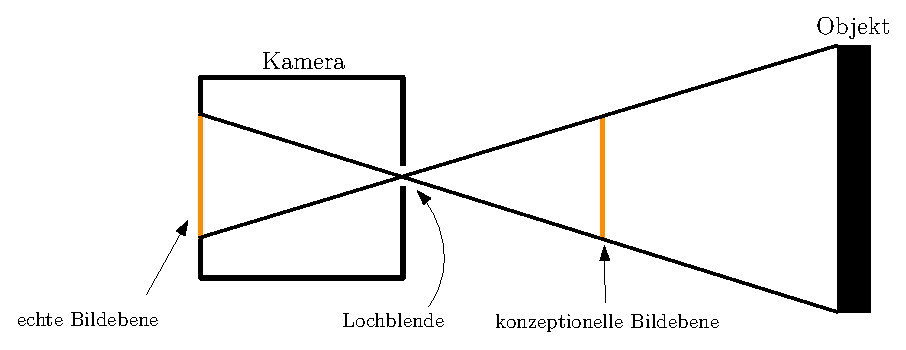
\includegraphics[scale=.8]{images/pinhole2.eps}
	\caption{Lochkameramodell}
	\label{fig:pinhole}
\end{figure}

Das Bild, das an der Rückseite der Kamera entsteht, ist dabei um 180° gedreht. Damit man diese Rotation nicht betrachten muss, kann man die Bildebene virtuell vor die Lochblende setzen. Da sich der Abstand zur Blende nicht ändert, ändern sich auch die optischen Eigenschaften des Bildes nicht.

Eine Kamerakalibrierung wird benötigt, um eine Beziehung zwischen Punkten im dreidimensionalen Weltkoordinatensystem und den Punkten auf der zweidimensionalen Bildebene herstellen zu können. Konkret wird eine projektive Abbildung

\begin{equation}\label{eq:projectionMat}
	\begin{pmatrix}
	wu \\wv \\w
	\end{pmatrix} =
		\underbrace{\begin{pmatrix}
		a_{11} & a_{12} & a_{13} & a_{14} \\
		a_{21} & a_{22} & a_{23} & a_{24} \\
		a_{31} & a_{32} & a_{33} & a_{34}
		\end{pmatrix}}_{=:A}	\begin{pmatrix}
		x \\y \\z \\ 1
		\end{pmatrix}
\end{equation}


gesucht, die einen Punkt $P=(x,y,z)$ in homogenen Koordinaten $\tilde P = (x,y,z,1)$ auf einen Punkt $\tilde C = (wu,wv,w)$ beziehungsweise nach der perspektivischen Division $C = (u,v)$ auf die Bildebene abbildet, wobei die $a_{ij}$ von den intrinsischen und extrinsischen Parametern der Kamera abhängen \cite{Heikkila1997}.

Als intrinsische Parameter einer Kamera werden die optischen Eigenschaften, sowie die interne Kamerageometrie bezeichnet. Hierzu zählen beispielsweise Linsenverzerrungen, sowie die Brennweite.
Extrinsische Parameter beschreiben die dreidimensionale Position und Orientierung der Bildebene relativ zu einem Weltkoordinatensystem  \cite{Tsai1987}.

%Man kann leicht zeigen, dass für $A$ gilt
%\[
%A = \lambda \cdot
%\begin{pmatrix}
%1 & 0 & u_0\\
%0 & 1 & v_0\\
%0 & 0 & 1
%\end{pmatrix}
%\begin{pmatrix}
%f & 0 & 0\\
%0 & f & 0\\
%0 & 0 & 1
%\end{pmatrix}
%\left(\begin{array}{ccc}
%R &  T\\
%0 & 1
%\end{array}\right) = \lambda\underbrace{\begin{pmatrix}
%f & 0 & u_0\\
%0 & f & v_0\\
%0 & 0 & 1
%\end{pmatrix}}_{=:V}
%\left(\begin{BMAT}(e)[1pt]{ccc|c}{ccc|c}
%& & & \\
%& \text{\large R}& & \text{\large T} \\
%& &  & \\
%0 & 0 & 0 & 1
%\end{BMAT}\right),
%\]
%
%wobei $\lambda$ ein beliebiger Skalierungsfaktor ist. $V$ beschreibt die intrinsischen und $R$ und $T$ die extrinsischen Parameter (siehe \cite{Heikkila1997}). $f$ ist hierbei die Brennweite; $(u_0, v_0)$ die Bildmitte.

%Zunächst wird also das Weltkoordinatensystem wie in Abbildung \ref{fig:extrinsic} mit einer Rotation und einer Translation in das Kamerakoordinatensystem überführt. Anschließend wird

Die Matrix $A$ kann mit gegebenen Punktkorrespondenzen bestimmt werden. Dafür werden Punkte $(x_k,y_k,z_k)$ für $k = 1,\dotsc,m$ im Weltkoordinatensystem und die korrespondierenden Punkte $(u_k, v_k)$ auf der Bildebene benötigt.
Zunächst wird das Gleichungssystems \ref{eq:projectionMat} nach $u$ und $v$ umgestellt:

\[
 \begin{aligned}
 u_k &= \frac{a_{11} x_k +a_{12}y_k + a_{13}z_k + a_{14}}{a_{31} x_k +a_{32}y_k + a_{33}z_k + a_{34}} \\
 v_k &= \frac{a_{21} x_k +a_{22}y_k + a_{23}z_k + a_{24}}{a_{31} x_k +a_{32}y_k + a_{33}z_k + a_{34}}.
 \end{aligned}
\]

Die Matrixeinträge $a_{ij}$ werden als Unbekannte betrachtet und das Gleichungssystem kann noch einmal umformuliert werden zu:

 \setcounter{MaxMatrixCols}{20}
\begin{equation}\label{eq:DLT}
\underbrace{\begin{pmatrix}
x_1 & y_1 & z_1 & 1 & 0 & 0 & 0 & 0 & -u_1 x_1 & -u_1 y_1 & -u_1z_1 \\
0 & 0 & 0 & 0 & x_1 & y_1 & z_1 & 1 & -v_1x_1 & -v_1y_1 & -v_1z_1 \\
\vdots & \vdots & \vdots & \vdots & \vdots & \vdots & \vdots & \vdots & \vdots & \vdots & \vdots\\
x_m & y_m & z_m & 1 & 0 & 0 & 0 & 0 & -u_m x_m & -u_m y_m & -u_m z_m \\
0 & 0 & 0 & 0 & x_m & y_m & z_m & 1 & -v_mx_m & -v_my_m & -v_mz_m
\end{pmatrix}}_{=:M}
\begin{pmatrix}
a_{11} \\ a_{12} \\ a_{13} \\ a_{14} \\ a_{21} \\ a_{22} \\ a_{23} \\ a_{24} \\ a_{31} \\ a_{32} \\ a_{33}
\end{pmatrix} =
\begin{pmatrix}
u_1 \\ v_1 \\ \vdots \\ u_m \\ v_m
\end{pmatrix},
\end{equation}

wobei $a_{34}$ auf eins skaliert werden darf, da in homogenen Koordinaten gerechnet wird. Es handelt sich hierbei für $m \geq 6$ um ein überbestimmtes lineares Gleichungssystem, was mittels der Methode der kleinsten Quadrate (siehe Kapitel \ref{s:LSQ}) und durch eine Singulärwertzerlegung gelöst werden kann.
Dieses Verfahren wird auch als Direct Linear Transformation (DLT) bezeichnet.

Das beschriebene Verfahren vernachlässigt dabei Linsenverzerrungen. Solche Verzerrungen entstehen entweder als Produktionsfehler günstiger Linsen, oder werden durch spezielle Linsen, wie bei Weitwinkelkameras, begünstigt. Verzerrungen können in der Regel nicht linear modelliert werden. Der Ansatz über DLT funktioniert hier dementsprechend nicht.

Es wird grundsätzlich zwischen zwei Typen von Verzerrungen unterschieden: radiale Verzerrung und tangentiale Verzerrung.
Radiale Verzerrung entsteht durch eine Skalierung des Abstands eines Bildpunktes zum Fokus. Wird der Abstand vergrößert, spricht man von einer tonnenförmigen Verzerrung (siehe Abbildung \ref{fig:barrel}), wird er verkleinert von einer kissenförmigen Verzerrung (siehe Abbildung \ref{fig:cushion}).

Radiale Verzerrung kann wie folgt modelliert werden:

\[
\begin{aligned}
\hat{x}^{(r)} &= x\left[1 + k_1\left(x^2 + y^2\right) + k_2\left(x^2 + y^2\right)^2 \right] \\
\hat{y}^{(r)} &= y\left[1 + k_1\left(x^2 + y^2\right) + k_2\left(x^2 + y^2\right)^2 \right],
\end{aligned}
\]

wobei $(x,y)$ ein verzerrter Bildpunkt, $(\hat{x}^{(r)}, \hat{y}^{(r)})$ der entzerrte Punkt und $k_1$ und $k_2$ die Koeffizienten der radialen Verzerrung sind \cite{Zhang2002}.

Tangentiale Verzerrung ist auf eine fehlerhafte Fertigung zurückzuführen und entsteht beispielsweise, wenn sich eine Linse nicht parallel zur Bildebene befindet.
Sie kann modelliert werden durch:
\[
\begin{aligned}
\hat{x}^{(t)} &= \left[2p_1xy + p_2\left((x^2 + y^2) + 2x^2\right)\right] \\
\hat{y}^{(t)} &= \left[p_1\left((x^2 + y^2) + 2y^2\right) + 2p_2xy\right],
\end{aligned}
\]

wobei $(x,y)$ wieder ein verzerrter Bildpunkt, $(\hat{x}^{(t)}, \hat{y}^{(t)})$ der entzerrte Punkt und $p_1$ und $p_2$ die Koeffizienten der tangentialen Verzerrung sind \cite{Heikkila1997}.

\begin{figure}[!htb]
	\centering
	\begin{subfigure}{.33\textwidth}
		\centering
		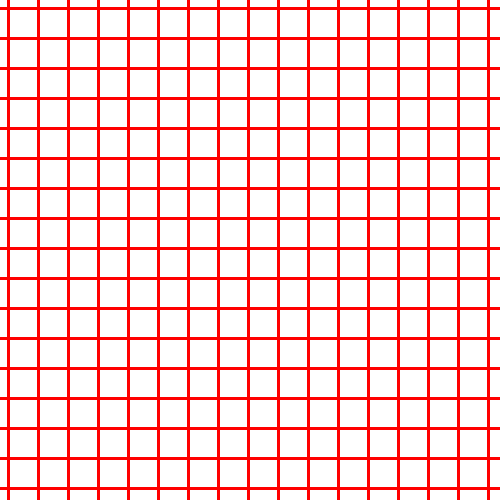
\includegraphics[width=0.9\textwidth]{images/undistorted.png}
		\caption{keine Linsenverzerrung}
		\label{fig:undist}
	\end{subfigure}%
	\begin{subfigure}{.33\textwidth}
		\centering
		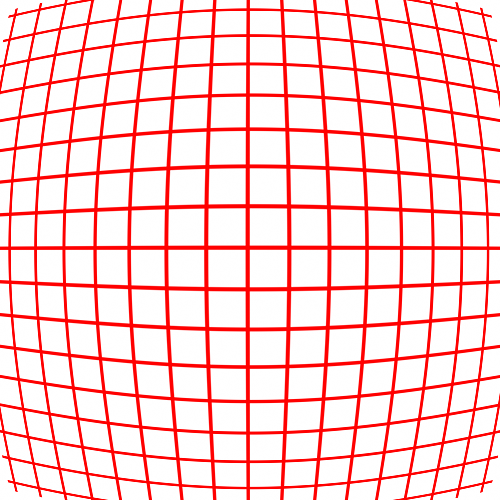
\includegraphics[width=0.9\textwidth]{images/barrelDistortion.png}
		\caption{tonnenförmige Verzerrung}
		\label{fig:barrel}
	\end{subfigure}%
	\begin{subfigure}{.33\textwidth}
		\centering
		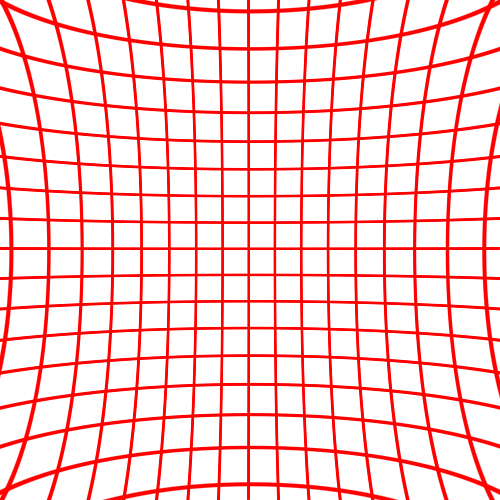
\includegraphics[width=0.9\textwidth]{images/cushionDistortion.png}
		\caption{kissenförmige Verzerrung}
		\label{fig:cushion}
	\end{subfigure}
	\caption{Linsenverzerrungen}
	\label{fig:distortion}
\end{figure}



\section{Blob-Detektor}
\label{s:blob}
\begin{definition}[Blob]\label{def:blob}
	Ein Blob ist eine glatte zusammenhängende Region in einem Bild, die sich farblich von ihrer Umgebung abhebt \cite{Lindeberg1993}.
\end{definition}

Ein Blob-Detektor ist ein Verfahren zum Detektieren solcher Blobs. Die gefundenen Blobs können anschließend unter anderem nach folgenden Kriterien gefiltert werden:
\begin{itemize}
	\item \textbf{Fläche} beschreibt die Größe eines Blobs
	\item \textbf{Rundheit} beschreibt die Ähnlichkeit zu einem Kreis und ist definiert durch $circ = \frac{4\pi\cdot \textrm{Fläche}}{\left(\textrm{Umfang}\right)^2}\in[0,1]$, wobei ein Kreis mit $circ = 1$ maximal rund ist.
	\item  \textbf{Konvexität} beschreibt die Ähnlichkeit eines Blobs zu seiner konvexen Hülle. Konvexität ist definiert als $conv = \frac{\textrm{Fläche Blob}}{\textrm{Fläche konvexe Hülle}}\in[0,1]$
\end{itemize}

%\section{Canny}
%\label{s:canny}
%Der Canny-Algorithmus \cite{Canny1986} ist ein Verfahren zur Kantendetektion. Im Gegensatz zu anderen Verfahren wie Sobel, oder Prewitt, versucht Canny die Fehlerrate der Kantendetektion minimal zu halten.
%Darüber hinaus markiert Canny die Kanten möglichst exakt, minimiert also die Distanz eines markierten Punktes zum eigentlich Zentrum der Kante.
%Zuletzt gewährleistet Canny außerdem die Eindeutigkeit einer Kante. Das bedeutet, dass eine Kante nicht mehrmals markiert wird.

\section{Hough-Transformation}
\label{s:hough}
Die Hough-Transformation ist ein Verfahren zur Detektion von beliebigen parametrisierbaren Konturen. In dieser Arbeit wird Hough-Transformation benutzt, um Geraden zu detektieren.

Eine beliebige zweidimensionale Gerade kann in Polarkoordinaten folgendermaßen implizit ausgedrückt werden:

\begin{equation}\label{eq:HoughLines}
x\cos\phi + y\sin\phi = d,
\end{equation}

wobei $\phi \in [0,2\pi)$ der Winkel der Geraden mit der $x$-Achse und $d \geq 0$ der Radius, also der euklidische Abstand der Geraden zum Ursprung des Koordinatensystems, ist.

Eine Gerade wird somit als ein Punkt $(d,\phi)$ in den Parameterraum (auch Hough-Raum) abgebildet.

Um eine Gerade eindeutig zu definieren benötigt man, wie auch bei der klassischen Definition $y = mx + b$, zwei Punkte. Beschränkt man sich auf einen Punkt, so lässt sich jedoch die Auswahl von $\phi$ und $d$ einschränken. Hat man beispielsweise einen Punkt $(x_k,y_k)$ gegeben, so ergibt die Gleichung \ref{eq:HoughLines} eine sinusförmige Funktion in Abhängigkeit von $\phi$.

Um nun beliebige Geraden detektieren zu können, werden $\phi$ und $d$ zunächst passend diskretisiert:
\[
	\begin{aligned}
		\phi_i &= \phi_{min} + \frac{i}{n} \cdot (\phi_{max} - \phi_{min}) \quad&\forall &i\in [0,n]\\
		d_j &= d_{min} + \frac{j}{m} \cdot  (d_{max} - d_{min}) &\forall &j\in [0,m]
	\end{aligned}
\]



Es wird nun ein Akkumulator $\mathcal{H}(\phi, d)$ für alle $\phi_i$ und $d_j$ auf null gesetzt.
Als Nächstes wird ein Kantenbild mittels Canny \cite{Canny1986} erzeugt. Die Kantenpixel werden mit $(x_k,y_k)$ für $k = 0,\dotsc,l$ identifiziert. Das eigentliche Verfahren funktioniert nach folgendem Schema:

\begin{algorithm}
	\caption{Hough-Transformation}\label{euclid}
	\begin{algorithmic}[1]
		\For{$k = 0 ~\textbf{to}~ l$} \Comment{für alle Kantenpunkte}
		\For{$i = 0 ~\textbf{to}~ n$} \Comment{für alle diskreten Winkel $\phi_i$}
		\State $d \gets x_k\cos\phi_i + y_k\sin\phi_i$
		\State $d_i \gets \textbf{round}(d)$ \Comment{runde $d$ zum nächsten diskreten $d_i$}
		\State  $\mathcal{H}(\phi_i, d_i) \gets \mathcal{H}(\phi_i, d_i) + 1$
		\EndFor
		\EndFor
	\end{algorithmic}
\end{algorithm}

\FloatBarrier
Die Werte im Akkumulator werden oft auch als Votes bezeichnet. Am Ende des Verfahrens wird im Akkumulator nach Häufungspunkten gesucht. Jeder Häufungspunkt steht dort für einen Geradenkandidaten.


%Zu einen gegebenen Pixel wir nun für alle diskreten Winkel $\phi_i$ ein Wert für $d$ ausgerechnet und auf den nächsten diskreten Wert $d_j$ gerundet. Anschließend wird im Akkumulator  $\mathcal{H}$ der Wert an der Stelle $(\phi_i, d_j)$ erhöht. Für jeden Kantenpunkt werden sinusförmige diskrete Funktionen in den Hough-Raum abgebildet. Die Werte im Akkumulator werden oft auch als Votes bezeichnet.
%Am Ende des Verfahrens such man im Akkumulator nach Häufungspunkten. Jeder Häufungspunkt steht dort für einen Geradenkandidaten.


\section{RANSAC}
\label{s:ransac}
Random Sample Consensus (RANSAC) \cite{Fischler1981} ist ein nicht-deterministisches robustes Verfahren zur Parameterschätzung eines Modells bei einer, möglicherweise durch starke Ausreißer gestörten Messreihe.
Im Gegensatz zu Verfahren, wie der Methode der kleinsten Quadrate, die versuchen eine optimale Lösung für alle Messdaten zu bestimmen, wird bei RANSAC nur eine Teilmenge der Messreihe genutzt.

Aus der Menge der Messdaten wird wiederholt zufällig die minimale Anzahl Messdaten ausgewählt, die nötig ist, um das Modell eindeutig zu beschreiben und es wird dann geprüft, wie gut das geschätzte Modell die restlichen Messdaten beschreibt.
Die Güte des Modells wird im Allgemeinen durch ein Distanzmaß, wie zum Beispiel der euklidische Abstand, berechnet.
Hat ein Messdatum eine vorher definierte Maximaldistanz zum geschätzten Modell nicht überschritten, wird es ins sogenannte Consensus Set des Modells aufgenommen.
Das Modell mit dem größten Consensus Set wird schließlich ausgewählt.

Die Anzahl der Punkte, die notwendig sind, um das Modell eindeutig zu beschreiben sei durch $k\in\mathbb{N}$ gegeben. Der relative Ausreißeranteil wird mit $\epsilon \in[0,1)$ bezeichnet.
Die Anzahl der Iterationen, die mindestens notwendig sind, um mit einer Wahrscheinlichkeit von $p \in [0,1)$, bei einem relativen Ausreißeranteil von $\epsilon$ und $k$ Punkten mindestens einmal eine ausreißerfreie Teilmenge der Messreihe zu erhalten, lässt sich dann nach \cite{Fischler1981} berechnen als:

\begin{equation}
n_{min} = \frac{\log{\left(1-p\right)}}{\log{\left(1-\left(1-\epsilon\right)^k\right)}}.
\end{equation}


\section{Ellipsen}
\label{s:ellipse}
\subsection{Definition}
\label{s:ellipseGeneral}

\begin{definition}[Ellipse]
	Eine Ellipse wird beschrieben durch diejenigen Punkte, deren Summe der Abstände zu zwei gegebenen Punkten $f_1$ und $f_2$ (Brennpunkte) konstant sind. Der Mittelpunkt der Verbindungslinie der beiden Brennpunkte wird als Zentrum der Ellipse bezeichnet (siehe Abbildung \ref{fig:ellipseDef}).
	Als Hauptachse $a$ wird die Länge der Verbindungslinie vom Mittelpunkt durch einen der Brennpunkte bis zum Scheitelpunkt ($V_1$ beziehungsweise $V_3$) der Ellipse bezeichnet. Die Länge der zu ihr rechtwinkligen Verbindungslinie durch den Mittelpunkt bis zu einem der anderen Scheitelpunkte ($V_2$ beziehungsweise $V_4$) wird Nebenachse $b$ genannt.
\end{definition}

\begin{figure}[!htb]
	\centering
	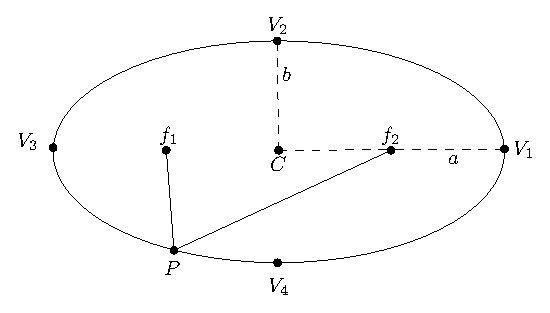
\includegraphics[scale=.9]{images/ellipse_focalDef.eps}
	\caption{Ellipse mit Brennpunkten $f_1/f_2$, Zentrum $C$, Hauptachse $a$, Nebenachse $b$ und Scheitelpunkten $V_1/V_3$ und $V_2/V_4$}
	\label{fig:ellipseDef}
\end{figure}

In ihrer einfachsten Form liegt die Ellipse im Zentrum des Koordinatensystems und ihre Haupt- und Nebenachse $a$ und $b$ sind achsenausgerichtet. Das heißt ihre Hauptachse liegt auf der $x$-Achse und ihre Nebenachse auf der $y$-Achse. Sie kann dann in der impliziten Form

\begin{equation} \label{eq:ellipseNoRotNoTrans}
\frac{x^2}{a^2} + \frac{y^2}{b^2} = 1
\end{equation}

beschrieben werden.

\begin{figure}[!htb]
	\centering
	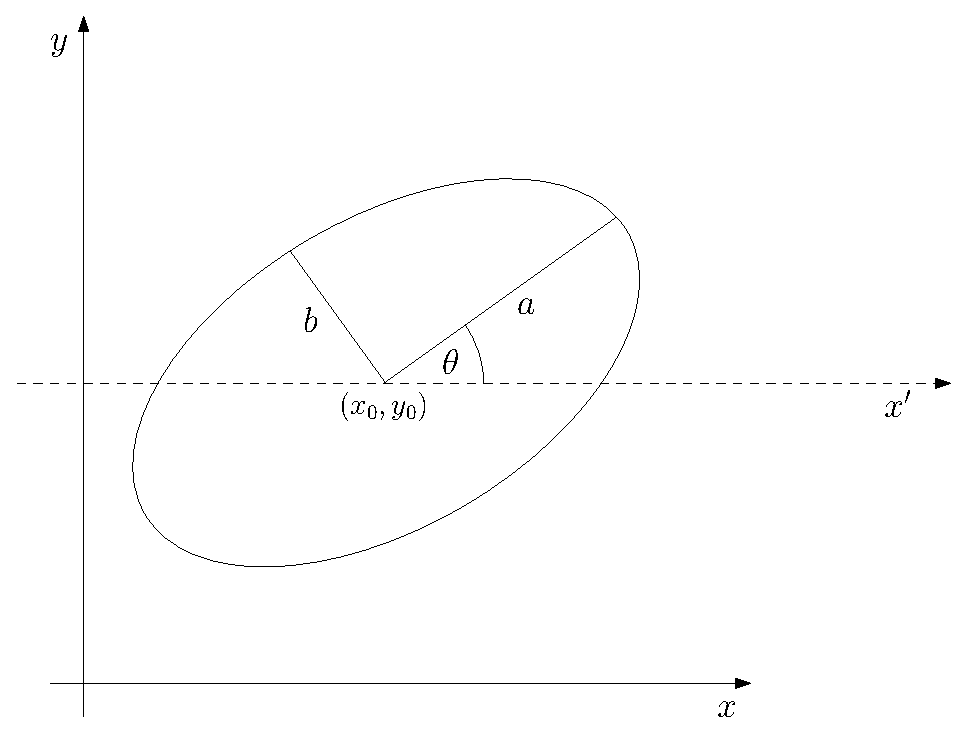
\includegraphics[scale=.7]{images/ellipse.eps}
	\caption{Ellipse mit Zentrum $(x_0, y_0)$, Hauptachse $a$, Nebenachse $b$, sowie Drehwinkel $\theta$}
	\label{fig:ellipse}
\end{figure}

Befindet sich die Ellipse nicht im Ursprung, so muss eine Verschiebung, beziehungsweise bei einer Rotation ein Drehwinkel (siehe Abbildung \ref{fig:ellipse}), ergänzt werden. Es gilt

\begin{equation} \label{eq:ellipseNoRotTrans}
\frac{\left(x-x_0\right)^2}{a^2} + \frac{\left(y-y_0\right)^2}{b^2} = 1
\end{equation}
für eine nicht rotierte Ellipse, beziehungsweise
\begin{equation} \label{eq:ellipseRotTrans}
\frac{((x - x_0)\cos\theta + (y - y_0)\sin\theta)^2}{a^2} + \frac{((x - x_0)\sin\theta - (y - y_0)\cos\theta)^2}{b^2} = 1
\end{equation}
für eine rotierte Ellipse mit Zentrum $(x_0,y_0)\in\mathbb{R}^2$, Hauptachsen $a,b\in\mathbb{R}^+$, sowie gegebenenfalls einem Drehwinkel $\theta \in [0,2\pi)$ oder parametrisiert

\begin{equation} \label{eq:ellipseRotTransParam}
\begin{pmatrix}x \\ y\end{pmatrix} = \begin{pmatrix}x_0 + a\cos\phi\cos\theta - b\sin\phi\sin\theta \\
y_0 + a\cos\phi\sin\theta + b\sin\phi\cos\theta\end{pmatrix}
\end{equation}
mit $\phi \in [0, 2\pi)$ und $x_0, y_0, a,b, \theta$ wie oben.

In ihrer allgemeinsten Form lässt sich eine Ellipse durch ein implizites Polynom zweiten Grades charakterisieren. Es gilt:
\begin{equation} \label{eq:ellipseQuadratic}
ax^2 + by^2 + cxy + dx + ey + f = 0 \quad \text{mit}\quad c^2-4ab < 0,
\end{equation}
wobei $a,b,c,d,e,f \in \mathbb{R}$. Eine Ellipse lässt sich demnach durch sechs Punkte eindeutig beschreiben (fünf, wenn man $f$ auf eins skaliert).


Die beiden Formen \ref{eq:ellipseRotTrans} und \ref{eq:ellipseQuadratic} sind äquivalent, falls die Ellipse nicht zu einem Punkt oder einer Linie degeneriert ist \cite{Lawrence1972}. Dies ist dann der Fall, wenn $a = b = 0$ (Punkt), oder $a = 0 \lor b = 0$ (Linie) gilt. Die Umformung von \ref{eq:ellipseRotTrans} nach \ref{eq:ellipseQuadratic} ist mit Hilfe einer Hauptachsentransformation möglich.
Da diese später benötigt wird, wird sie hier exemplarisch vorgeführt.

Zunächst einmal fällt auf, dass der gemischte Term $cxy$ genau dann null ist, wenn die Ellipse nicht rotiert wurde. Im ersten Schritt wird also die Rotation der Ellipse rückgängig gemacht, um den Rotationswinkel bestimmen zu können.

Die Gleichung \ref{eq:ellipseQuadratic} kann umgeformt werden zu:
\[
\begin{aligned}
&ax^2 + \frac{c}{2}xy + \frac{c}{2}yx + by^2 + dx + ey + f = 0 \\
\Leftrightarrow\quad &\begin{pmatrix}ax +  \frac{c}{2}y & \frac{c}{2}x + by\end{pmatrix}\begin{pmatrix}x \\ y\end{pmatrix} +  dx + ey + f = 0\\
\Leftrightarrow\quad &\underbrace{\begin{pmatrix}x & y\end{pmatrix}}_{=:u^T}\underbrace{\begin{pmatrix}a & \frac{c}{2} \\ \frac{c}{2} & b\end{pmatrix}}_{=: M}\underbrace{\begin{pmatrix}x \\ y\end{pmatrix}}_{=u} +\begin{pmatrix}d & e\end{pmatrix}\underbrace{\begin{pmatrix}x \\ y\end{pmatrix}}_{=u}+ f = 0 \\
\Leftrightarrow\quad &u^TMu +\begin{pmatrix}d & e\end{pmatrix}u + f = 0 \\
\end{aligned}
\]
Der gemischte Term wird alleine durch $M = \begin{pmatrix}a & \frac{c}{2} \\ \frac{c}{2} & b\end{pmatrix}$ bestimmt. Die Matrix $M$ ist invertierbar, denn
\[
\det M = ab - \dfrac{c^2}{4}
\] ist nur dann gleich null, wenn $c^2 - 4ab = 0$, was ein Widerspruch zur Annahme in Gleichung \ref{eq:ellipseQuadratic} ist. $M$ hat somit eine von null verschiedene Determinante und somit vollen Rang, hat also zwei von null verschiedene Eigenwerte \cite{Bosch2006}. Insbesondere gibt es zwei Eigenvektoren von $M$, die zueinander orthogonal sind, da Eigenvektoren zu verschiedenen Eigenwerten orthogonal zueinander sind.\cite{Bosch2006}.

Da die Matrix $M$ außerdem symmetrisch ist, ist sie orthogonal diagonalisierbar \cite{Bosch2006}.

Es gilt $M = S^TDS$, wobei $S\in\mathbb{R}^{2\times2}$ eine orthogonale Matrix mit den normierten Eigenvektoren als Zeilen und $D = \text{diag}(\lambda_1, \lambda_2)\in\mathbb{R}^{2\times2}$ eine Diagonalmatrix mit den beiden Eigenwerten von $M$ auf der Diagonalen ist. Ohne Beschränkung der Allgemeinheit gelte $\lambda_1 <= \lambda_2$, andernfalls werden die Eigenvektoren in $S$ vertauscht.

Sei nun $v := Su$.
So gilt:

\begin{equation} \label{eq:PCARot}
\begin{aligned}
&u^T(S^TDS)u +\begin{pmatrix}d & e\end{pmatrix}\underbrace{(S^TS)}_{=\ind}u + f = 0 \\
\Leftrightarrow\quad &(Su)^TD(Su) +\begin{pmatrix}d & e\end{pmatrix}S^T(Su) + f = 0 \\
\Leftrightarrow\quad &v^{T}Dv +\begin{pmatrix}d & e\end{pmatrix}S^Tv + f = 0 \\
\Leftrightarrow\quad &\lambda_1v_1^2 + \lambda_2v_2^2 +\begin{pmatrix}d & e\end{pmatrix}S^Tv + f = 0
\end{aligned}
\end{equation}

mit $v = (v_1,v_2)^T$. Man sieht, dass der gemischte Teil somit eliminiert wurde. Durch Anwenden der Transformation $S$ wurde $u$ in das Koordinatensystem, in dem die Ellipse achsenausgerichtet ist,  transformiert.

Eine Rotationsmatrix mit Rotationswinkel $\theta$ ist definiert durch:
\begin{equation}
\begin{aligned}
R = \begin{pmatrix}\cos\theta & -\sin\theta \\ \sin\theta & \cos\theta\end{pmatrix}
\end{aligned}
\end{equation}

Es gilt offenbar $S = R$ für ein geeignetes $\theta$, da die Eigenvektoren normiert und orthogonal zueinander sind. Mit der Funktion $\atant$ kann $\theta$ einfach ausgerechnet werden, denn es gilt:

\[
\theta = \atant(\sin\theta, \cos\theta) = \atant(S_{2,1}, S_{1,1})
\]

Formt man nun Gleichung \ref{eq:PCARot} weiter um, ergibt sich:

\begin{equation}\label{eq:ellipseCenter}
\begin{aligned}
&\lambda_1v_1^2 + \lambda_2v_2^2 + \underbrace{\begin{pmatrix}d & e\end{pmatrix}S^T}_{=:(d', e')}v + f = 0 \\
\Leftrightarrow\quad &\lambda_1v_1^2 + \lambda_2v_2^2 + d'v_1 + e'v_2 + f = 0 \\
\Leftrightarrow\quad &(\lambda_1v_1^2 + d'v_1)+ (\lambda_2v_2^2 + e'v_2) + f = 0\\
\Leftrightarrow\quad &(\lambda_1v_1^2 + d'v_1) + (\frac{d'^2}{4\lambda_1} - \frac{d'^2}{4\lambda_1}) + (\lambda_2v_2^2 + e'v_2) + (\frac{e'^2}{4\lambda_2} - \frac{e'^2}{4\lambda_2}) + f = 0 \\
\Leftrightarrow\quad &\left[\lambda_1\left(v_1^2 + \frac{2d'}{2\lambda_1}v_1 + \frac{d'^2}{4\lambda_1^2}\right) - \frac{d'^2}{4\lambda_1}\right] +\left[\lambda_2\left(v_2^2 + \frac{2e'}{2\lambda_2}v_2 + \frac{e'^2}{4\lambda_2^2}\right) - \frac{e'^2}{4\lambda_2}\right] + f = 0 \\
\Leftrightarrow\quad &\lambda_1(v_1 + \underbrace{\frac{d'}{2\lambda_1}}_{ = -x'_0})^2 +\lambda_2(v_2 + \underbrace{\frac{e'}{2\lambda_2}}_{ = -y'_0})^2 - \underbrace{\left(\frac{d'^2}{4\lambda_1} + \frac{e'^2}{4\lambda_2} - f\right)}_{=:\sigma} = 0,
\end{aligned}
\end{equation}

da $\lambda_1, \lambda_2 \neq 0$.

Das Zentrum der transformierten Ellipse $(x'_0, y'_0)$ kann nun aus Gleichung \ref{eq:ellipseCenter} abgelesen werden.
Um das Zentrum der eigentlichen Ellipse zu bestimmen, muss mit der inversen Rotation $S^T$ multipliziert werden:
\[
\begin{pmatrix} x_0 \\ y_0 \end{pmatrix} = S^T \begin{pmatrix} x'_0 \\ y'_0 \end{pmatrix}.
\]

Die Gleichung \ref{eq:ellipseCenter} lässt sich anschließend weiter vereinfachen:

\begin{equation} \label{eq:PCAKoeff}
\begin{aligned}
&\lambda_1(v_1 -x'_0)^2 +\lambda_2(v_2 -y'_0)^2 = \sigma \\
\Leftrightarrow\quad & \frac{\lambda_1}{\sigma}(v_1 -x'_0)^2 +\frac{\lambda_2}{\sigma}(v_2 -y'_0)^2  =1
\end{aligned}
\end{equation}

wobei $\sigma \neq 0$, wenn die Ellipse nicht zum Punkt entartet ist (folgt aus dem Determinantenkriterium \cite{Lawrence1972}). Aus dem Vergleich der beiden Gleichungen \ref{eq:PCAKoeff}, sowie \ref{eq:ellipseNoRotTrans} kann folgende Beziehung hergestellt werden:

\begin{equation}
\begin{aligned}
&\frac{\lambda_1}{\sigma} = \frac{1}{a^2} &\text{und}\quad &\frac{\lambda_2}{\sigma} = \frac{1}{b^2}\\
\Leftrightarrow\quad & \sqrt{\frac{\sigma}{\lambda_1}}  = a  &\text{und}\quad & \sqrt{\frac{\sigma}{\lambda_2}}  = b
\end{aligned}
\end{equation}

Das Ergebnis für die beiden Achsen ist reell, da $\frac{\sigma}{\lambda_i} > 0$ für nicht entartete reelle\footnote{Man kann Ellipsen auch mit imaginären Achsen definieren \cite{Lawrence1972}.}  Ellipsen gilt (folgt aus dem Determinantenkriterium \cite{Lawrence1972}). Da die Transformation in das Koordinatensystem der Ellipse nur Rotationen enthält,  bleiben die Längen der Hauptachsen erhalten. Es gilt wie erwartet $a \geq b$, da $\lambda_1 \leq \lambda_2$.


\subsection{Abstand: Punkt zu Ellipse}
\label{sc:distPointEllipse}
Das hier beschriebene Verfahren zur Bestimmung der kürzesten euklidischen Distanz eines Punktes zu einer Ellipse stammt aus der Arbeit von David Eberly \cite{Eberly2013}.
Es werden hierbei nur Ellipsen im Ursprung betrachtet, die achsenausgerichtet sind und darüber hinaus nur Punkte im ersten Quadranten. Ansonsten wird die Ellipse in den Ursprung verschoben und um ihren entgegengesetzten Drehwinkel rotiert.
Der untersuchte Punkt wird anschließend analog zur Ellipse transformiert.
Da die Ellipse dann bezüglich der $x$- und $y$- Achse symmetrisch ist, kann der Punkt einfach durch Spiegelung in den richtigen Quadranten verschoben werden. Der Abstand zur Ellipse ändert sich dadurch nicht.

Sei $Q = (x_1, y_1)$ ein Punkt, dessen Distanz zur Ellipse berechnet werden soll und $E = (x_0, y_0)$ derjenige eindeutige Punkt, welcher auf der Ellipse liegt und die kürzeste euklidische Distanz zum Punkt $Q$ hat.

Aufgrund dieser Forderungen können ohne Beschränkung der Allgemeinheit folgende Aussagen getroffen werden:
\begin{itemize}
	\item Die Ellipse kann stets durch die implizite Gleichung
	\begin{equation}\label{eq:distEqParam} \frac{x_0^2}{a^2} + \frac{y_0^2}{b^2} = 1\end{equation}
	 mit $a \geq b \geq 0$ beziehungsweise
	in der parametrischen Form
	\[
	\mathcal{E}(\phi) = (a\cos\phi, b\sin\phi) \quad \text{mit}\quad \phi \in [0, 2\pi)
	\] %%
	beschrieben werden.
	\item Es gilt $x_0,y_0,x_1,y_1 \geq 0$.
\end{itemize}

Für die quadratische Distanz von einem beliebigen Punkt $Q$ zu einem Punkt $\mathcal{E}(\phi)$ auf der Ellipse gilt dann
\begin{equation}
	F(\phi) = \left(\mathcal{E}(\phi) - Q\right)^2.
\end{equation}

Die Funktion $F$ soll bezüglich $\phi$ minimiert werden. Dazu muss ihre Ableitung betrachtet werden:
\begin{equation}\label{eq:perp}
F'(\phi) = 2\left(\mathcal{E}(\phi) - Q\right) \cdot \mathcal{E}'(\phi).
\end{equation}

$F'$ wird null, wenn $\left(\mathcal{E}(\phi) - Q\right)$ und $ \mathcal{E}'(\phi)$ zu einander orthogonal sind. Daraus folgt, dass der Vektor von $Q(x_1,y_1)$ zu $E(x_0,y_0)$ senkrecht zur Ellipse stehen muss (siehe Abbildung \ref{fig:ellipseDist}).


\begin{figure}[!htb]
	\centering
	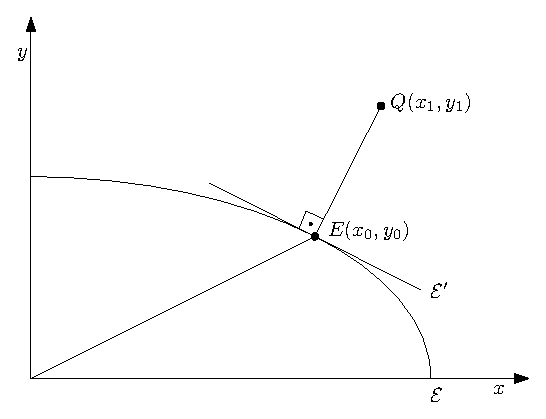
\includegraphics[scale=.9]{images/ellipseQuery.eps}
	\caption[Ellipsenausschnitt im ersten Quadranten mit Abfragepunkt $Q$ und eingezeichneter kürzester Distanz zum Ellipsenpunkt $E$]{Ellipsenausschnitt im ersten Quadranten mit Abfragepunkt $Q$ und eingezeichneter kürzester Distanz zum Ellipsenpunkt $E$. Die Ellipse wird beschrieben durch $\mathcal{E}$}
	\label{fig:ellipseDist}
\end{figure}

Die Nullstellen der Funktion
\begin{equation} \label{eq:ellipseDistEq}
	G(x,y) = \frac{x^2}{a^2} + \frac{y^2}{b^2} - 1,
\end{equation}
basierend auf der impliziten Darstellung aus Gleichung \ref{eq:distEqParam},
beschreiben eine Ellipse. Sei nun solch eine Nullstelle gegeben durch $(x_0,y_0)$. Der Gradient $\nabla G$ ist dann in $(x_0,y_0)$ ein Normalenvektor der Ellipse. Somit ist auch der halbe Gradient\footnote{nutzt man den halben Gradienten kürzen sich das $1/2$ und die $2$ aus den partiellen Ableitungen der Ellipse heraus} $\nabla G(x_0,y_0)/2$ ein Normalenvektor. Da aus Gleichung \ref{eq:perp} die Orthogonalität von $\overrightarrow{QE}$ zur Ellipse folgt,  muss der Vektor  $\overrightarrow{QE}$ ein skalares Vielfaches des halben Gradienten sein. Es gilt somit:

\begin{equation}
	(x_1,y_1) - (x_0, y_0) = t\frac{\nabla G(x_0,y_0)}{2} = t\left(\frac{x_0}{a^2},\frac{y_0}{b^2}\right)
\end{equation}
für ein $t\in\mathbb{R}$.

Umgestellt nach $x_1$ und $y_1$, beziehungsweise nach $x_0$ und $y_0$, ergeben sich folgende Gleichungen:

\begin{equation}\label{eq:ellipseDistY}
x_1 = x_0\left(1 + \frac{t}{a^2}\right), \quad y_1 = y_0\left(1 + \frac{t}{b^2}\right)
\end{equation}

\begin{equation}\label{eq:ellipseDistX}
x_0 = \frac{a^2x_1}{t+a^2},\quad y_0 = \frac{b^2y_1}{t+b^2}
\end{equation}


\bigskip
Man macht nun eine Fallunterscheidung:
\begin{enumerate}
	\item Der einfachste Fall ist, wenn sich der Punkt $Q$ auf der $y$-Achse (außer $(0,0)$) befindet, wenn also gilt $x_1 = 0, y_1 > 0$.
	Da die Hauptachse nach der $x$-Achse ausgerichtet ist und $a \geq b$ gilt, ist der Punkt auf der Ellipse mit der kürzesten Distanz zu $Q$ offenbar $E = (0, b)$ und für die Distanz gilt $d = \abs{y_1 - b}$.
	\item Als nächstes befinde sich $Q$ auf der $x$-Achse (einschließlich $(0,0)$), wenn also gilt  $x_1 \geq 0, y_1 = 0$. Es gilt mit \ref{eq:ellipseDistY}
	\begin{equation} \label{eq:xAxisQ}
		x_1 = x_0\left(1 + \frac{t}{a^2}\right), \quad 0 = y_0\left(1 + \frac{t}{b^2}\right)
	\end{equation}

	Wenn $y_0 = 0$ gilt, muss $x_0 = a$ gelten, damit $E(x_0,y_0)$ auf der Ellipse ist. Es  gilt analog zum ersten Fall $E=(a,0)$ mit $d = \abs{x_1 - a}$

	Gilt $y_0 \neq 0$, so kann in der zweiten Gleichung aus Gleichung \ref{eq:xAxisQ} durch $y_0$ geteilt werden und es folgt $t = -b^2$ und somit $x_1 = x_0\left(1 - \frac{b^2}{a^2}\right)$. Der Punkt $E(x_0,y_0)$ liegt außerdem oberhalb von $(a,0)$ und es gilt deshalb auf Grund der Krümmung der Ellipse $x_0 < a$.

	Insgesamt ergibt sich mit Gleichung \ref{eq:ellipseDistX} die Ungleichung
	\[
	\begin{aligned}
		&x_0 = \frac{a^2x_1}{a^2 - b^2} < a \\
		\Leftrightarrow\quad &x_1 < \frac{a^2 - b^2}{a} < a.
	\end{aligned}
	\] %%

	Das bedeutet, dass sich der Punkt $Q(x_1,y_1)$ in der Ellipse befindet.

	Für Punkte $Q(x_1,0)$ mit $x_1 \geq \frac{a^2 - b^2}{a}$ muss dementsprechend $y_0 = 0$ gelten und der kürzeste Punkt ist wieder $E(a,0)$.

	Für Punkte $Q(x_1,0)$ mit $x_1 < \frac{a^2 - b^2}{a}$ muss für $E(x_0,y_0)$, nach Umstellen der Ellipsengleichung \ref{eq:distEqParam},~$y_0 = b\cdot\sqrt{1-\left(\frac{x_0}{a}\right)^2}$ gelten.
	Die quadratische Distanz von $E(x_0,y_0)$ zu $Q(x_1,0)$ beträgt dann:
	\[
		d^2 = (x_0 - x_1)^2 + (y_0 - 0)^2.
	\] %%
	Setzt man nun $y_0 = b\cdot\sqrt{1-\left(\frac{x_0}{a}\right)^2}$ ein und für jedes Vorkommen von $x_0$ die Gleichung $x_0 = \frac{a^2x_1}{a^2 - b^2}$ ein, so ergibt sich insgesamt:
	\[
	\begin{aligned}
	d^2 &= (x_0 - x_1)^2 + (y_0 - 0)^2 \\
	&= \left(x_1\frac{a^2}{a^2-b^2} - x_1\right)^2 + b^2\left(1 - x_1^2\frac{a^2}{(a^2-b^2)}\right) \\
	&= x_1^2\left(\frac{a^2}{a^2-b^2} - 1\right)^2 - b^2x_1^2\frac{a^2}{\left(a^2-b^2\right)^2} + b^2 \\
	&= x_1^2\left[\frac{a^4}{\left(a^2-b^2\right)^2} - 2\frac{a^2}{a^2-b^2} + 1 - \frac{b^2a^2}{\left(a^2-b^2\right)^2}\right] + b^2\\
	&= x_1^2\left[\frac{a^4 - 2a^2(a^2-b^2) + \left(a^2-b^2\right)^2 - b^2a^2}{\left(a^2-b^2\right)^2}\right] + b^2\\
	&= x_1^2\left[\frac{a^4 - 2a^4 + 2a^2b^2 + a^4 -2a^2b^2 + b^4 - b^2a^2}{\left(a^2-b^2\right)^2}\right] + b^2\\
	&= x_1^2\left[\frac{b^4-b^2a^2}{\left(a^2-b^2\right)^2}\right] + b^2 = x_1^2\left[\frac{-b^2\left(a^2-b^2\right)}{\left(a^2-b^2\right)^2}\right] + b^2 \\
	&= -b^2\frac{x_1^2}{a^2-b^2} + b^2 = b^2\left(1-\frac{x_1^2}{a^2-b^2}\right).\\
	\end{aligned}
	\] %%
	\item Der letzte Fall ist der allgemeinste Fall. Es gilt $x_1 > 0$, sowie $y_1 > 0$. Da sich laut Voraussetzung alle Punkte im ersten Quadranten befinden, gilt darüber hinaus $x_0, y_0 \geq 0$. Mit diesen Eigenschaften und Gleichung \ref{eq:ellipseDistY} lässt sich folgende Einschränkung für $t$ herleiten:
\[
	\begin{aligned}
	& 0 < x_1 = x_0\left(1 + \frac{t}{a^2}\right)\\
	\Leftrightarrow\quad& 0 < 1 + \frac{t}{a^2} \\
	\Leftrightarrow\quad& -1\cdot a^2 < t.
	\end{aligned}
\]
	Analog ergibt sich mit $y_1\colon -b^2 < t$. Da $a\geq b$ gilt, reicht es nur die zweite Ungleichung zu betrachten, da sie die erste impliziert. Setzt man nun Gleichung \ref{eq:ellipseDistX} in Gleichung \ref{eq:ellipseDistEq} ein, erhält man:

\[
	\begin{aligned}
		F(t) &= \left(\frac{a^2x_1}{a\left(t+a^2\right)}\right)^2 + \left(\frac{b^2y_1}{b\left(t+b^2\right)}\right)^2 - 1 \\
		&= \left(\frac{ax_1}{t+a^2}\right)^2 + \left(\frac{by_1}{t+b^2}\right)^2 - 1
	\end{aligned}
\]

	Durch Untersuchung der Ableitungen kann nun gezeigt werden, dass diese Funktion auf dem gesamten Intervall $[-b^2,\infty)$ monoton fällt und links gekrümmt ist \cite{Eberly2013}. Darüber hinaus gilt:
	\[
	\lim\limits_{t \searrow -b^2}{F(t)}	= +\infty, \quad\lim\limits_{t \rightarrow \infty}{F(t)}	= -1.
	\]
	Da $F$ stetig ist, muss es eine Nullstelle geben, die aufgrund des Monotonie- und Krümmungsverhaltens sogar eindeutig ist. Die Nullstelle lässt sich beispielsweise durch Intervallschachtelung oder dem Newton-Verfahren bestimmen.
\end{enumerate}


\section{Analytical Deformable Templates}
\label{s:anaDef}
Analytical Deformable Templates ist ein Verfahren zur Detektion von analytischen Kurven.
Ein Template ist dabei definiert durch eine Menge von Parametern, die a-priori Wissen über die erwartete Form ermöglichen.
Als Beispiel sei eine  Ellipse genannt, die durch ihr Zentrum, ihren beiden Achsen und den Drehwinkel, also $(x_0,y_0,a,b,\theta)$ definiert ist.
Es wird dann eine Energiefunktion konstruiert, deren Terme eine Anziehung des Templates an Hauptmerkmale (wie Kantenstärke, Kantenorientierung, Farbintensität, etc. ) des Bildes hervorrufen.
Die Energiefunktion wird dabei durch numerische Verfahren, wie dem Gradientenverfahren, minimiert \cite{Yuille1992}.
